% --------------------------------------------------------------
%                           Set Up
% --------------------------------------------------------------
 
\documentclass[12pt]{article}
 
\usepackage[margin=1in]{geometry} 
\usepackage{amsmath,amsthm,amssymb}
\usepackage{listings}
\usepackage{xcolor}
\usepackage{graphicx}
\usepackage{subcaption}
\usepackage{listings}
\usepackage{xcolor}
\usepackage{comment}
\usepackage{hepnames}
\usepackage{longtable}
 
\definecolor{codegreen}{rgb}{0,0.6,0}
\definecolor{codegray}{rgb}{0.5,0.5,0.5}
\definecolor{codepurple}{rgb}{0.58,0,0.82}
\definecolor{backcolour}{rgb}{0.95,0.95,0.92}
 
\lstdefinestyle{mystyle}{
    backgroundcolor=\color{backcolour},   
    commentstyle=\color{codegreen},
    keywordstyle=\color{magenta},
    numberstyle=\tiny\color{codegray},
    stringstyle=\color{codepurple},
    basicstyle=\ttfamily\footnotesize,
    breakatwhitespace=false,         
    breaklines=true,                 
    captionpos=b,                    
    keepspaces=true,                 
    numbers=left,                    
    numbersep=5pt,                  
    showspaces=false,                
    showstringspaces=false,
    showtabs=false,                  
    tabsize=2
}
 
\lstset{style=mystyle}
 
\definecolor{codegreen}{rgb}{0,0.6,0}
\definecolor{codegray}{rgb}{0.5,0.5,0.5}
\definecolor{codepurple}{rgb}{0.58,0,0.82}
\definecolor{backcolour}{rgb}{0.95,0.95,0.92}
\definecolor{deepblue}{rgb}{0,0,0.5}
\definecolor{deepred}{rgb}{0.6,0,0}
\definecolor{deepgreen}{rgb}{0,0.5,0}
 
\lstdefinestyle{mystyle}{
    backgroundcolor=\color{backcolour},   
    commentstyle=\color{codegreen},
    keywordstyle=\color{deepred},
    numberstyle=\tiny\color{codegray},
    stringstyle=\color{deepblue},
    basicstyle=\ttfamily\footnotesize,
    breakatwhitespace=false,         
    breaklines=true,                 
    captionpos=b,                    
    keepspaces=true,                 
    numbers=left,                    
    numbersep=5pt,                  
    showspaces=false,                
    showstringspaces=false,
    showtabs=false,                  
    tabsize=2
}
 
\lstset{style=mystyle}
 
\newcommand{\N}{\mathbb{N}}
\newcommand{\Z}{\mathbb{Z}}
 
\newenvironment{theorem}[2][Theorem]{\begin{trivlist}
\item[\hskip \labelsep {\bfseries #1}\hskip \labelsep {\bfseries #2.}]}{\end{trivlist}}
\newenvironment{lemma}[2][Lemma]{\begin{trivlist}
\item[\hskip \labelsep {\bfseries #1}\hskip \labelsep {\bfseries #2.}]}{\end{trivlist}}
\newenvironment{exercise}[2][Exercise]{\begin{trivlist}
\item[\hskip \labelsep {\bfseries #1}\hskip \labelsep {\bfseries #2.}]}{\end{trivlist}}
\newenvironment{problem}[2][Problem]{\begin{trivlist}
\item[\hskip \labelsep {\bfseries #1}\hskip \labelsep {\bfseries #2.}]}{\end{trivlist}}
\newenvironment{question}[2][Question]{\begin{trivlist}
\item[\hskip \labelsep {\bfseries #1}\hskip \labelsep {\bfseries #2.}]}{\end{trivlist}}
\newenvironment{corollary}[2][Corollary]{\begin{trivlist}
\item[\hskip \labelsep {\bfseries #1}\hskip \labelsep {\bfseries #2.}]}{\end{trivlist}}

\newenvironment{solution}{\begin{proof}[Solution]}{\end{proof}}

\setlength\parindent{0pt}
 
\begin{document}
 
% -------------------------------------------------------------- 
%                         Start here
% --------------------------------------------------------------
 
\title{Homework 1}
\author{Timothy Holmes\\ %replace with your name
PHY 442 Computational Physics}

\maketitle

\section*{Problem 1}

To be able to solve for the cubic spline later in the assignment, the tridiagonal system needs to be addressed. The tridiagonal system tends to be in the form found in Equation 2.19 in the text. The coefficents a, b, and c as well as the fight hand side vector can be extracted from this system. The extracted values are all of the know values in the system. The unknown values in the system are x values in the vector being multiplied by the matrix A. From the prior equation the values become what we find in equation 2.21,

$$
\beta_{1} = b_{1}, \beta_{j} = b_{j} - \frac{a_{j}}{\beta_{j - 1}}c_{j - 1} \;\;\;\; j = 2,...,N 
$$

and equation 2.22,

$$
\rho_{1} = r_{1}, \rho{j} = r_{j} - \frac{a_{j}}{\beta{j - 1}}\rho_{j - 1} \;\;\;\; j = 2,...,N 
$$

The x values can be found from $x_{N - 1}$ and reworking the equations above, the x values are found from equation 2.23,

$$
x_{N - j} = \frac{\rho_{N - j} - c_{n - j}x_{N - j + 1}}{\beta_{N - j}} \;\;\;\; j = 1,...,N.
$$

With the data gave in Homework 1, the code tridiagonal system in the appendix is used to find the following values;

\begin{align*}
x1 = 3.33, \\
x2 = 6.67, \\
x3 = 9.00, \\
x4 = 9.33, \\
x5 = 6.67.
\end{align*}

\section*{Problem 2}

The idea of the cubic spline to to try and "fit" a cubic between each set of data points x and y. Essentially, the idea is to fill in those missing points between the data points. A cubic spline is fitting the polynomial

$$
p(x) = a_{j}(x - x_{j})^{3} + b_{j}(x - x_{j})^{2} + c_{j}(x - x_{j}) + d_{j}; \;\;\;\; x_{j} \leq x \leq x_{j + 1}.
$$

Using and following the logic in the appendix code Cubic Spline Program, the following chart is produced. 

\begin{figure}[h!]
    \centering
    {{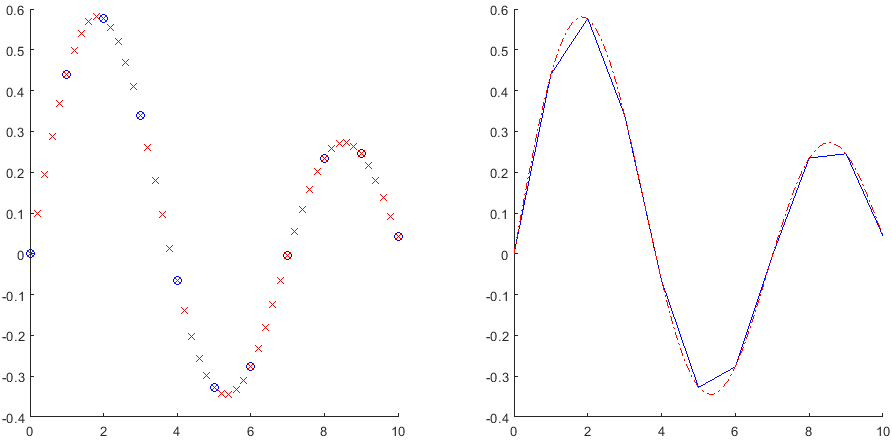
\includegraphics[width=15cm]{figure1.png}}}%
    \qquad
    \caption{Problem 2: A fit polynomial using data from Homework 1. }%
    \label{fig:example}%
\end{figure}


\section*{Problem 3}

This problem required a slight change from tthe prior problem. In this problem we are given fake derivative data. Using this data, since we know the derivatives $p'_{1}$ and $p'_{N}$, we can use equation 2.17 and solve the problem. Using this data produces the following graph below. The output data can also be found in the table in the appendix.

\begin{figure}[h!]
    \centering
    {{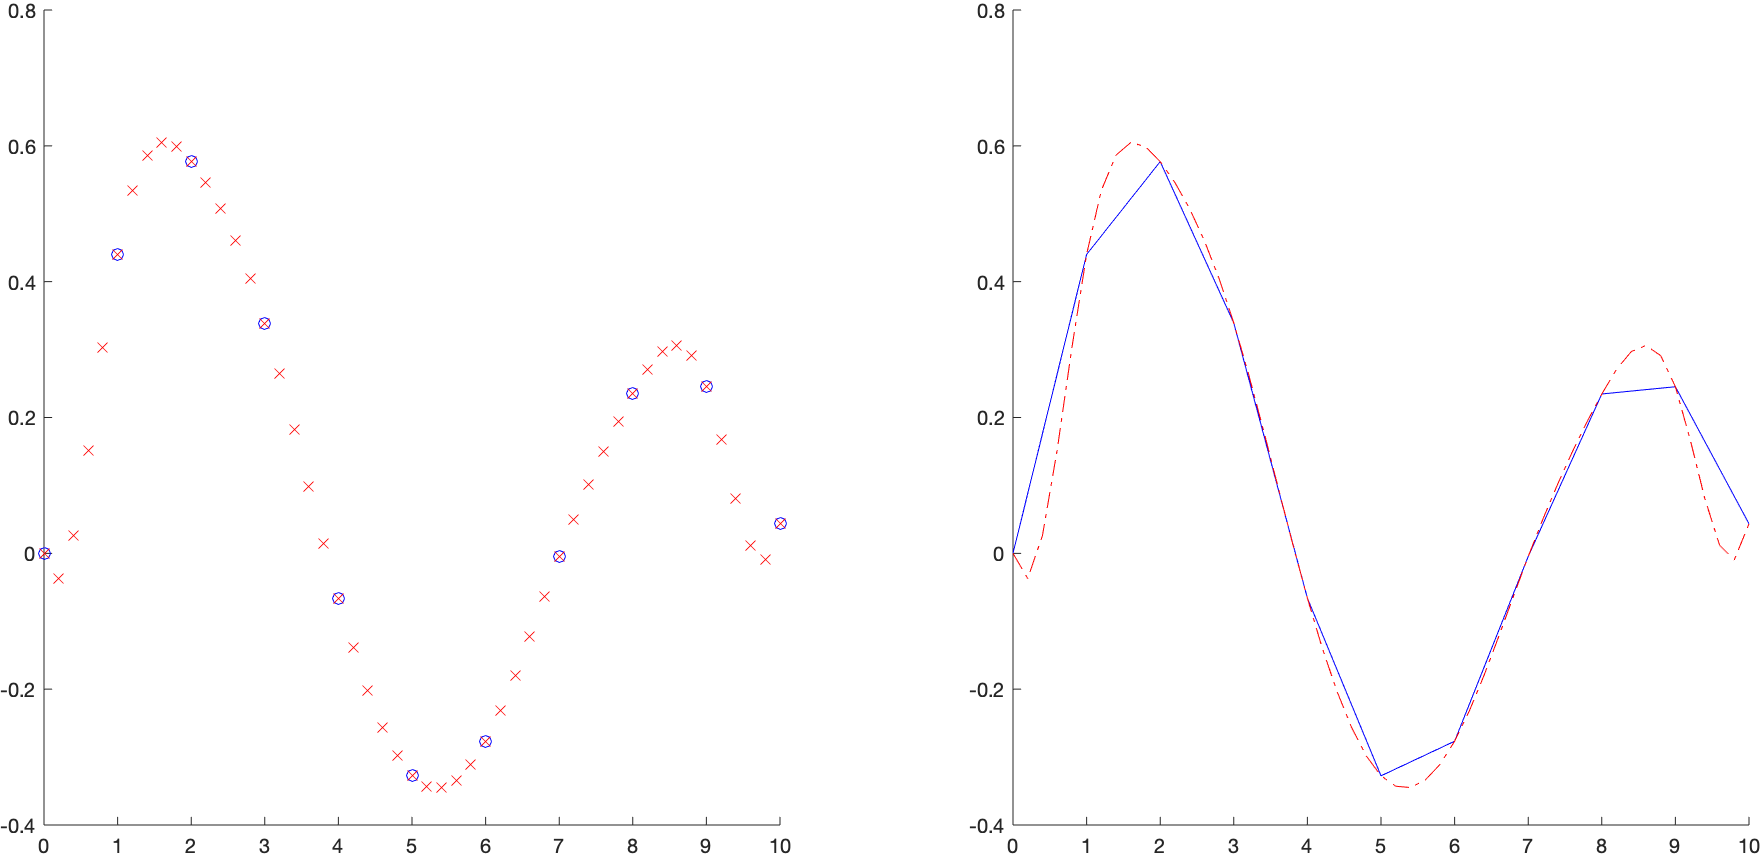
\includegraphics[width=15cm]{figure2.png}}}%
    \qquad
    \caption{Problem 3 A fit polynomial using data from Homework 1 and the fake derivative values.}%
    \label{fig:example}%
\end{figure}


It is hard to tell if there are any differences when comparing figure 1 and figure 2. But there are some considerable changes when comparing bot graphs. If we look at the first data point, figure 1 shows the curve fitted data going straight from point 1 to point 2. However, figure 2 shows that the curve fit data dips below the first point and then moves up to point 2. Then the next point, figure 1 curve fit data never plots above the third point. However, the curve fit data in figure 2 does plot above the third point. We again see very similar issues with the tailing data. Overall, bot graphs are very similar.

\newpage

\section*{Appendix}

\subsection*{Tridiagonal System}
\begin{lstlisting}[language=Matlab, caption=Tridiagonal Program]
function tridiagonal_system(A, r)
%% Tridiagonal Program
%   - Find unkown x_i values while knowing the
%     matrix and r.h.s array
%   
%   Input Arg
%   ---------
%   A - martix:
%       A general tridiagonal system.
%   r - array:
%       R.H.S values.

%   Optional Input
%   --------------
%   None
%       Runs func that rutens homework 1 Args
%
%   Output Arg
%   ----------
%   None - prints unknow x_i values to console
%
%   Modify for output arg, change function to:
%       [x] = function tridiagonal_system(A, r)

if (~exist('A', 'var')) && (~exist('r', 'var'))
    [A, r] = homework_1_values(); 
end

%% Define variables   
N = length(A);          % Returns largest array dim in matrix
a = [(0); diag(A, -1)]; % diag at first col second row
b = diag(A);            % diag of matix
c = [diag(A, 1); 0];    % diag of second col first row

% Preallocate beta, rho
beta = zeros(1, N);
rho  = zeros(1, N);

%% Run calculations
% Initial values are beta_1 = b_1 and rho_1 = r_1
beta(1)  = b(1);
rho(1)   = r(1);

for j = 2:N
    beta(j) = b(j) - a(j)/beta(j - 1) * c(j - 1);
    rho(j)  = r(j) - a(j)/beta(j - 1) * rho(j - 1);
end

% Final row of matrix
x(N) = rho(N) / beta(N);

% Repeat for all row
for j = 1:N-1
    x(N - j) =  (rho(N - j) - c(N - j) * x(N - j + 1)) / beta(N - j);
end

%% Output values
count = 1:length(x);
fprintf("The x values are:\n")
fprintf("-----------------\n")
fprintf("|   x%d = %0.2f   |\n", [count(:), x(:)].')
fprintf("-----------------\n")

end


function [A, r] = homework_1_values()
A = [ 2 -1   0   0  0; -1  2  -1   0  0; 0 -1   2  -1  0; 0  0  -1   2 -1; 0  0   0  -1  2;];
r = [0; 1; 2; 3; 4;];
end
\end{lstlisting}


\subsection*{Cubic Spline Program}
\begin{lstlisting}[language=Matlab, caption=Cubic Spline Program]
function [p_x] = cubic_spline(x, y, spacing)
%% Cubic Spline
%   - Curve fit
%   
%   Input Arg
%   ---------
%   x - array: Default: Homework 1 values
%       x-axis values of a table/plot.
%   y - array: Default: Homework 1 values
%       y-axis values of a table/plot
%   spacing - int: Optional argument: Default: 5
%       Number of curve fit plot point between 
%       (x, y) and (x + 1, y + 1).
%
%   Optional Input
%   --------------
%   None
%       Runs func that rutens homework 1 Args
%
%   Output Arg
%   ----------
%   p_x - Curve fit plots
%   x   - Original x-axis values

if (~exist('x', 'var')) && (~exist('y', 'var'))
    [x, y] = homework_1_values(); 
end

%% Preallocate 
n = length(x);
A = zeros(n, n);
h = zeros(n, 1);
r = zeros(n - 2, 1);

%% Calculate h, matrix A, and R.H.S values
for i = 1:(n - 1)
   h(i) = x(i + 1) - x(i);
end
for i = 2:(n - 1)
    A(i, (i - 1):(i + 1)) = [h(i ) 2 * (h(i - 1) + h(i)) h(i + 1)];
end
for i = 1:(n - 2)
   r(i) = (6 * (y(i + 2) - y(i + 1)))/h(i + 1) - (6 * (y(i + 1) - y(i)))/h(i); 
end

%% Set matrix for a natural cubic spline
r           = [0; r; 0;];
A(2, 1)     = 0;
A(1,1)      = 1;
A(n, n)     = 1;

%% Call trisolve, return second derivative (p'') as (p)
p = trisolve(A, r);

%% Preallocate 
p_x = zeros(n, 1);
a   = zeros(n, 1); b = zeros(n, 1);
c   = zeros(n, 1); d = zeros(n, 1);

%% Calculate Coefficents 
for j = 1:(n - 1)
   a(j) = (p(j + 1) - p(j))/(6 * h(j));
   b(j) = p(j)/2;
   c(j) = (y(j + 1) - y(j))/h(j) - (h(j) * p(j + 1))/6 - (h(i) * p(j))/3;
   d(j) = y(j);
end

%% Default Spacing - set up curve fit plots
if (~exist('spacing', 'var'))
    spacing = 5;
end

x_step  = (x(2) - x(1))/spacing;
dx      = x(1):x_step:x(end);


%% Calculate ploynomial 
for i = 1:(n - 1)
    for j = ((spacing * (i - 1)) + 1):(spacing * (i) + 1)
        p_x(j) = a(i) * (dx(j) - x(i))^3 + b(i) * (dx(j) - x(i))^2 + c(i) * (dx(j) - x(i)) + d(i);
    end
end

p_x = p_x';

%% Plot
set(gcf, 'Position', [100 100 1100 500])
subplot(1, 2, 1)
hold on
plot(x, y, 'bo')
plot(dx, p_x, 'rx')

subplot(1, 2, 2)
hold on
plot(x, y, 'b-')
plot(dx, p_x, 'r-.')


end




function [x, y] = homework_1_values()
rho = [0; 1; 2; 3; 4; 5; 6; 7; 8; 9; 10;];
J_0 = [1.00000; 0.76519; 0.22389; -0.26005; -0.39714; -0.17759; 0.15064; 0.30007; 0.17165; -0.09033; -0.24593];
J_1 = [0.00000; 0.44005; 0.57672; 0.33905; -0.06604; -0.32757; -0.27668; -0.00468; 0.23463; 0.24531; 0.04347;];
J_2 = [0.00000; 0.11490; 0.35283; 0.48690; 0.36412; 0.04656; -0.24287; -0.30141; -0.11299; 0.14484; 0.25463;];
J_1_prime = (J_0 - J_2)/2;
J_1_prime_hardcode = -3:0.5:3;

x = rho;
y = J_1;
end
\end{lstlisting}

\begin{longtable}{| c | c | c |}
\hline
index & x & p(x) \\
\hline
1 & 0.000000 & 0.000000 \\ 
2 & 0.200000 & 0.099151 \\ 
3 & 0.400000 & 0.195516 \\ 
4 & 0.600000 & 0.286311 \\ 
5 & 0.800000 & 0.368751 \\ 
6 & 1.000000 & 0.440050 \\ 
7 & 1.200000 & 0.497782 \\ 
8 & 1.400000 & 0.540951 \\ 
9 & 1.600000 & 0.568921 \\ 
10 & 1.800000 & 0.581057 \\ 
11 & 2.000000 & 0.576720 \\ 
12 & 2.200000 & 0.555702 \\ 
13 & 2.400000 & 0.519501 \\ 
14 & 2.600000 & 0.470041 \\ 
15 & 2.800000 & 0.409250 \\ 
16 & 3.000000 & 0.339050 \\ 
17 & 3.200000 & 0.261525 \\ 
18 & 3.400000 & 0.179386 \\ 
19 & 3.600000 & 0.095500 \\ 
20 & 3.800000 & 0.012736 \\ 
21 & 4.000000 & -0.066040 \\ 
22 & 4.200000 & -0.138181 \\ 
23 & 4.400000 & -0.201936 \\ 
24 & 4.600000 & -0.255772 \\ 
25 & 4.800000 & -0.298160 \\ 
26 & 5.000000 & -0.327570 \\ 
27 & 5.200000 & -0.342873 \\ 
28 & 5.400000 & -0.344552 \\ 
29 & 5.600000 & -0.333490 \\ 
30 & 5.800000 & -0.310571 \\ 
31 & 6.000000 & -0.276680 \\ 
32 & 6.200000 & -0.232950 \\ 
33 & 6.400000 & -0.181508 \\ 
34 & 6.600000 & -0.124731 \\ 
35 & 6.800000 & -0.064996 \\ 
36 & 7.000000 & -0.004680 \\ 
37 & 7.200000 & 0.053939 \\ 
38 & 7.400000 & 0.108971 \\ 
39 & 7.600000 & 0.158624 \\ 
40 & 7.800000 & 0.201108 \\ 
41 & 8.000000 & 0.234630 \\ 
42 & 8.200000 & 0.257720 \\ 
43 & 8.400000 & 0.270195 \\ 
44 & 8.600000 & 0.272193 \\ 
45 & 8.800000 & 0.263852 \\ 
46 & 9.000000 & 0.245310 \\ 
47 & 9.200000 & 0.217017 \\ 
48 & 9.400000 & 0.180675 \\ 
49 & 9.600000 & 0.138294 \\ 
50 & 9.800000 & 0.091888 \\ 
51 & 10.000000 & 0.043470 \\ 
\end{longtable}


% --------------------------------------------------------------
%                           End Document.
% --------------------------------------------------------------
 
\end{document}

